\section{The Scanner, Parser and Chosen Parser Generator Tool}
This chapter will explain what the job of the scanner and parser is in compiler construction, what a parsing generator tool is, the theories it implements and which parser generator we chose for Ezuino.
% \begin{figure}[H]
%\centering
%\includegraphics[width=\textwidth]{figures/compiler-process.png}
%\caption{Organization of a compiler, Source: Fischer \cite{crafting-a-compiler} }
%\label{syntax-overview}
%\end{figure}
%This chapter will contain the decisions we made in regards to the compiler of our language, as well as our arguments for making these decisions.

\subsection{The Scanner}
A scanner, also called a Lexer, is the first processing step of a programming language. It reads the input text, ignores comments, and turns it into a compact and uniform format known as tokens.
A scanner is most often created through declarative programming, often done with the parser generator tool. That it is declarative means to create the scanner you tell the generator what tokens to recognize in regular expressions and let the generator do the implementation.

\label{parsing-subsubsection}
\subsection{Parsing}
Just like the scanner, a parser is often created through declarative programming by a parsing generator tool. The purpose of the parser is to read tokens generated by the scanner and generate phrases according to a context-free grammar file, which then checks are syntactically correct. If there is an error it either reports it, attempts to repair it (to create a syntactically valid program), or tries to recover from the error in order to continue parsing. Besides verifying the syntax of a program is valid, the parsing should also generate a concrete syntax tree. This concrete syntax tree can then create an abstract syntax tree used by other parts of the compiler.

\subsection{Choosing a parser generator tool}
In order to understand what the parser generator tool does, it is necessary to explain the theory behind parsing techniques. When constructing a parser one of two strategies is usually used to recognize and construct tokens based on the context-free grammar of the language, namely top-down parsing and bottom-up parsing. It is also necessary to keep in mind what kind of parsing the generated parser does. Finally, the different generator tools create a concrete parse tree and how easy they are to convert to an abstract syntax tree should also be taken into consideration.
\subsubsection*{Top-down and bottom-up parsing}
Given a starting symbol and a set of rules, a top-down parser will start reading its input as a long line of tokens from a scanner. In general, the tokens are read from left to right\footnote{Unless your source language is a language that writes from right to left, of course}, and are afterwards derived from the starting symbol using a leftmost-derivation of the non-terminals through the grammatical rules\cite{conceptsOfProgrammingLanguages}.\\
\\
An example of a top-down parsing is the recursive descent parser, which is built from a collection of subprograms that each produces its own top-down parse tree generator. The subprograms in itself are recursive and the recursive descent parser will only create one subprogram for every non-terminal it can find in the user-generated grammar\cite{conceptsOfProgrammingLanguages}.\\
\\
A bottom-up parser is the other method of parsing. A bottom-up parser also reads a line of tokens, but rather than starting at the top and deriving to terminals, it builds non-terminals based on the symbols it reads, by performing a rightmost-derivation in accord with the grammatical rules, until it reaches the starting symbol\cite{conceptsOfProgrammingLanguages}.\\
\\
\subsubsection{Parsing trees and abstract parsing tree}
The end goal of either strategy is to generate a parse tree\footnote{Sometimes known as a concrete syntax tree (a CST)}, which represents the syntactic structure of the program source code. The parse tree is defined by an input string and a grammar, or in this case for the project, a context-free-grammar \\

\begin{figure}[H]
\centering
\caption{Parse tree example}
\label{exampleparse}
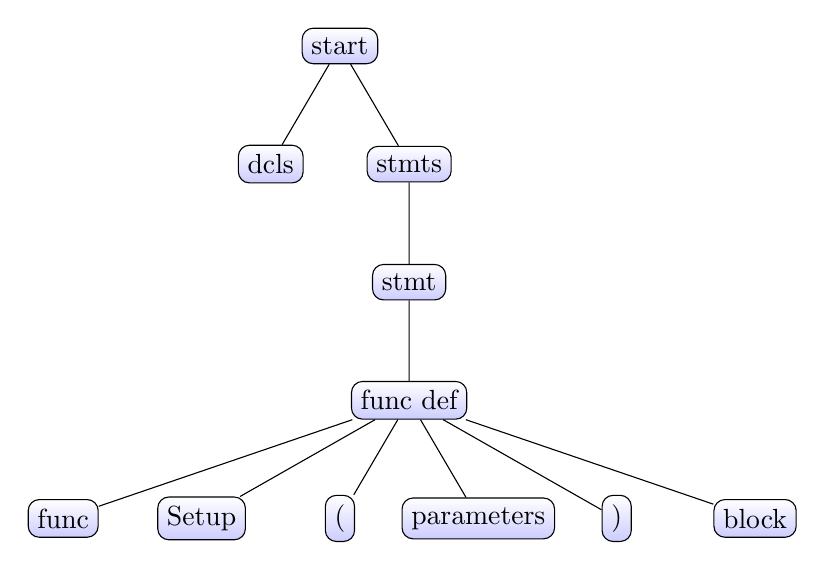
\begin{tikzpicture}[sibling distance=5em,
  every node/.style = {shape=rectangle, rounded corners,
    draw, align=center,
    top color=white, bottom color=blue!20}]]
  \node {start}
    child { node {dcls} }
    child { node {stmts}
      child { node {stmt}
        child { node {func def}
          child { node {func} }
          child { node {Setup} }
          child { node {(} }
          child { node {parameters} }
          child { node {)} } 
          child { node {block} } } } };
\end{tikzpicture}
\end{figure}

The picture in figure \ref{exampleparse} shows a parse tree, where the highest node, which is “start” has 2 child nodes which are “dcls” and “stmts”. It will then traverse further down until it reaches an end. \\
An abstract syntax tree provides the advantage that removes non-essential elements of the syntax. E.g. the colons, equality signs etc. and provides a structure which can be altered and annotated to make sure that contextual analysis is performed correctly.
The abstract syntax tree is more an idea since it is very dependent on the construction of the programming language. The structure is a representation of the essential information from the parse tree, with inessentials removed (braces, parentheses, etc.). In an abstract syntax tree the entire source program should be stored in the structure and using this structure alone, the compiler programmer should be able to reconstruct the entire source program. If one cannot recreate the source program, essential structures have been removed.\cite{crafting-a-compiler}
A common method of creating an abstract syntax three is through the visitor pattern. The visitor pattern is an object oriented pattern provided by the GoF Design Patterns book.
It solves the problem of defining a new operation without changing the classes of the elements on which it operates.
The visitor therefore makes it easy to handle methods in a class in a specific context. A visitor simply has to specify how to visit all the nodes in the tree.
\subsubsection{Types of parsing}
\subsubsection*{LL-parsing}
The LL parser (Left to right and left most derivation) is a parser that parses its input from left to right while using a top-down parsing technique. It is usually denoted as LL(k), where k is a greater than or equal to 0, where the k signifies the amount of lookahead tokens the parser can look at\cite{conceptsOfProgrammingLanguages}.

\subsubsection*{LR-parsing}
The LR parser (Left to right and rightmost derivation) is a parser that parses its input from left to right, but unlike the LL(k) parser, the LR parser uses a bottom-up parsing technique and produces a rightmost derivation. Just as the LL(k) the k in the LR(k)-definition signifies the amount of tokens the LR will look ahead for\cite{conceptsOfProgrammingLanguages}. LR-parsers usually have a magnitude of either 0 or 1 (LR(0) or LR(1)), as LR(1)-parsers already use many resources to parse a given input, and even higher magnitudes severely slow down the entire program.

\subsubsection*{LALR- and LALR(1) parsing}
The LALR(k) parser is a parser that utilizes the same parsing strategy as the LR(k) parser (bottom-up), but with a different way to generate a parse table, the part of an LR parser that instructs the parser how to react to a given input. Usually, an LALR-parser is of magnitude 1, as an LALR(1)-parser is more powerful than an LR(0)-parser and by powerful it means that it can modify more language\cite{crafting-a-compiler}, but not as resource intensive as an LR(1)-parser. It should be noted, that the LR(1)-parser is still more powerful than the LALR(1)-parser, which is why it is still in use\cite{crafting-a-compiler}.

\subsubsection*{Table driven LL(K) parsing}
The table driven LL(k) parser uses a similarity analysis to the generated grammar so that when it starts with pushing the start symbol into the stack, the parser would try to find a match of symbols from the input and when found, put the symbol into the top of the stack\cite{crafting-a-compiler}. This is nice for when you have a big code block and you want the parsing to be automated by using a stack.

\subsubsection{Considered parser generators and choice}
In this subsection we will list the different parser generator tools we tried and which one we chose. \\

\begin{table}[h]
\centering
\begin{tabular}{@{}ll@{}}
\toprule
\textbf{Parser} & \textbf{Type} \\ \midrule
ANTLR           & LL(*)         \\
Bison           & LALR(1)       \\
GOLD            & LALR(1)       \\
SableCC         & LALR(1)       \\ \bottomrule
\end{tabular}
\label{parser_table}
\end{table}

\noindent
Out, of all the possible generators we researched, we seriously considered two of them. \\
\\
One of them was using a tool called Flex, an open-source implementation of the Lex program for generating a scanner and Bison, a Yacc-based parser generator, for generating a parser. To get familiar with the tools, we attempted to implement an infix calculator. It was not particularly complex to use the tools together, but it was not always clear why an error occurred, due to the unfamiliar naming scheme that bison and flex use. \\
Flex and Bison only target C and C++, meaning we would also have to write the rest of our compiler in C or C++. While both C and C++ are powerful languages, it is also hard to write well, and it takes a long time to write code that works. \\
The other alternative which is also the one we chose, was ANTLR4. ANTLR4 targets Java is comparative more efficient and which we were more familiar with. The naming convention used by the ANTLR4 parser made more sense as well, and the context free grammar format for ANTLR4 was also slightly more practical. Another advantage of ANTLR4 was that it also generates a base abstract syntax tree interface that can be extended by the programmer. This helped setting up the structure of the abstract syntax tree. ANTLR4 is also more popular and was therefore also easier to find documentation for.








%\subsection{Type Checker}
%During the Type Checker, the types of variables and functions are checked. By saving what the type of each variable is, it is possible to check whether the variables are correctly used. This might be to check if an assignment of the variable is possible or not. This phase is not limited to only type checking. The phase is meant for all the semantic analysis, which is dependant on the compiler programmers. This might include checking for double declaration, declaration before usage, etc.
%The result of running the Type Checker is a decorated Abstract Syntax Tree. The abstract syntax tree might is decorated with types but might have other information associated with it, depending on the compiler.

%\subsection{Translator and optimizer}
%The translator phase of the compiler takes the decorated abstract syntax tree and makes it into an intermediate representation. The reason for this is that it might be easier to deal with the intermediate representation in the code generation phase.
%The translator phase is optional as code can be generated directly from the abstract syntax tree.
%The output result is simply the intermediate representation.
%The optimizer phase is optional. This is where the code is optimized and bottlenecks are removed. It is done with the idea in mind that you can reduce the size of the code and also reduce the running time of the program. 

%\begin{itemize}
%    \item Peekhole optimization
%    \item Constant folding
%    \item Common sub-expression elimination
%    \item Code motion
%    \item Dead code elimination
%\end{itemize}{}

%In order to make more efficient code one might eliminate dead variables like this:
%\begin{verbatim}
%func int magicNumber() {
%    int t
%    t := 40 * 20 - 100 / 4
%    return 42
%}
%\end{verbatim}
%where t is a dead variable.




%\subsection{Code Generator}
%In the Code Generator phase, the target code is generated. Depending if the compiler generated the intermediate representation or not, the source here is either the intermediate representation or the abstract syntax tree directly. The implementation here is very dependant on the target language as some target languages uses registers directly or stack based machines.

%ANTLR4 only provides a context syntax tree (also known as a parse tree) of the source program. The parse tree from ANTLR is the direct translation of the source program parsed by ANTLR using the grammar. The nodes in the parse tree is thus directly related to the tokens provided in the grammar.

%To convert the parse tree to an abstract syntax tree, you have to convert every single node to the alternative.
%Doing this with ANTLR requires a great overview of both datastructures and the visitor which can be generated by ANTLR. The visitor is an ANTLR specific implementation of the visitor pattern.



%\subsection{Symboltable}
%While the visitor pattern provides a way of handling the nodes in the abstract syntax tree there might be necessary to keep some information when transitioning trough the nodes. This can simply be kept in a private attribute for simple information. However there might be some difficulty dealing when scope rules. Thus it might be nessecary with a symboltable.
%A symboltable is datastructure that XX TODO. Whenever opening a new scope the symboltable needs to know and thus declares a new scope. Whenever exiting a scope, close the scope. 
%You end up with a decorated abstract syntax tree.

%\subsubsection{Codegeneration}
%earing the end, of the compiler, after doing all the contextual analysis, you end up with a decorated syntax tree which has made sure that everything lives up to the programming language that has been defined. Now it’s time for code generation.
%Here there can be multiple code generators as it simply can follow the visitor pattern in order to generate the code. This is the point where the designer of the compiler decides what the resulting language of the compiler should be. It could be C, Assembly, etc. It depends on what the programming language is designed for. Sometimes it might be necessary to make some predefined code in order to support the structures and functionality of the programming language.
%A good approach might be to create an intermediate language if you want to compile multiple high-level programming languages to a low-level programming language. In that way instead of making many compilers from D => B, E => B, D => C, E => C, you can simply create one compiler from the high-level language to the intermediate language. Similarly, if you want to output to multiple low level languages, you simply need to add another compiler from the intermediate language to the new low-level language. In that way, instead of making high-level \* low-level number of compilers, you simply have to make Highlevel \+ Low-level number of compilers. It adds abstraction but might also add complexity if either the source language or the destination language has structures which are hard or impossible to implement. Some examples of compilers with intermediate languages are Java and C\#. Java compiles to Java Bytecode which is the instruction set of the Java Virtual Machine. C\# compiles to Common Intermediate Language which is then run on the Common Language Runtime.

%\subsection{Compiler}
%A compiler is a translator from a source language to a target language.
%Depending on the compiler, the compiler may generate one or more of these: Pure Machine Code, Augmented Machine Code or Virtual Machine Code.[Ref Fischer]
%In this report the source language is the language "Ezuino" and the target language is Jasmin [TODO].

%\subsubsection{Jasmin}
%Jasmin is an assembler for the Java Virtual Machine. It provides takes ASCII syntax of the Java Bytecode and makes into the binary Java Bytecode. [Fischer cap 10.2.2]. 
